\documentclass[11pt,letterpaper]{article}

%%%%%%%%%%%%%%%%%%%%%%%%%%%%%%%%%%%%%%%%%%%%%%%%%%%%%%%%%%%%%%%%%%%%%%%%%
\pagestyle{plain}                                                      %%
%%%%%%%%%% EXACT 1in MARGINS %%%%%%%                                   %%
\setlength{\textwidth}{6.5in}     %%                                   %%
\setlength{\oddsidemargin}{0in}   %% (It is recommended that you       %%
\setlength{\evensidemargin}{0in}  %%  not change these parameters,     %%
\setlength{\textheight}{8.5in}    %%  at the risk of having your       %%
\setlength{\topmargin}{0in}       %%  proposal dismissed on the basis  %%
\setlength{\headheight}{0in}      %%  of incorrect formatting!!!)      %%
\setlength{\headsep}{0in}         %%                                   %%
\setlength{\footskip}{.5in}       %%                                   %%
%%%%%%%%%%%%%%%%%%%%%%%%%%%%%%%%%%%%                                   %%
\newcommand{\required}[1]{\section*{\hfil #1\hfil}}                    %%
\renewcommand{\refname}{\hfil References Cited\hfil}                   %%
%\bibliographystyle{plain}                                              %%
%%%%%%%%%%%%%%%%%%%%%%%%%%%%%%%%%%%%%%%%%%%%%%%%%%%%%%%%%%%%%%%%%%%%%%%%%

%PUT YOUR MACROS HERE

\usepackage{amsmath}
\usepackage{amsfonts}
\usepackage{amssymb}
\usepackage{graphicx}
\usepackage{ulem}
\usepackage{placeins}

%\renewcommand{\thesection}{\Roman{section}} 
%\renewcommand{\thesubsection}{\thesection.\Roman{subsection}}

\title{NMR}

\date{}

\author{Ian Hunt-Isaak}


\begin{document}


\maketitle
\begin{abstract}
Using a TeachSpin Pulsed NMR PS1-D device we determined the spin relaxation constants $T_1$ and $T_2$ for a sample of mineral oil using standard techniques. The values were determined to be $T_1=21.68\pm 1.2$ ms and $T_2=6.25\pm .55$ ms. It is speculated that the sample is better described by multiple $T_1$ times and suggestions for future work investigating that idea are developed. The theory and usage of NMR are also discussed.
\end{abstract}
\section{Introduction}
Nuclear Magnetic Resonance known as NMR observes the transition between different spins states of protons placed in an external magnetic field. It is excellent as a technique to understand the local environment of atoms in a molecule. Therefore it is standard technique in use in Chemistry Labs today. For an excellent listing of the modern uses of NMR see Ref. \cite{NMR_Uses}. 

Originally discovered by Isidor Isaac Rabi, NMR was independently developed into a very useful technique by Felix Bloch,  and Edward Purcell in the 1940s. Since then powerful computers have dramatically increased its utility from a tool for nuclear physics to a standard chemistry technique.
In this experiment we use NMR as a basic tool to determine the two characteristic times of a system. A static magnetic field will be used unlike in the modern usage of NMR in Chemistry in which a sweep of fields are used, for more information on the usage of NMR in bulk matter see Ref. \cite{Pake}. This experiment provides the basis information for a more complete analysis of the structure of mineral oil and serves more as a demonstration of concept than a useful technique as the implications of the calculated characteristic times in not discussed.
\section{Background and Theory}
In this experiment we apply an external magnetic field along the Z axis, see Fig. \ref{fig:Sample_Env}. Due to the quantization of the spin of a proton nuclei will be forced into one of two magnetic energy states separated by $\Delta U=\hbar\omega_o$ with $\omega_o$ as the processional frequency of the magnetic moment of the nucleus around the $Z$ axis.

In NMR we are concerned with measuring the the behavior of Hydrogen Nuclei magnetic moments under an externally applied constant magnetic field in order to learn about the local field environments of the protons in the sample. When an external magnetic field is applied in the direction of the $+Z$ axis, see Fig. \ref{Sample_Env}, there will be two possible magnetic energy states for each proton, each state associated with spin $+\frac{1}{2}$ or $-\frac{1}{2}$. These states have the the proton's magnetic moment is either aligned or anti-aligned with the external field $B_0$ have an energy separation of $\Delta U=\hbar\omega_o$ with $\omega_o$ as the processional frequency of the magnetic moment of the nucleus around the $Z$ axis, $\omega_o$ is dependent on $B_0$. Any changes in the local field environment of a proton will cause the $\Delta U$ for the proton to be shifted relative to the other protons. In order to study these variations in field environment spins are flipped away from the $+Z$ direction and the time it takes them to return to this more energetically favorable state is recorded allowing us to glean information on the different local field environment for protons in the material.

By the application of an oscillating magnetic field $B_1$ along the X-axis the direction the spins of the protons can be flipped from $+Z$ to $-Z$, 180 degrees, or 90 degrees from the Z axis to the transverse (x-y) plane. We describe the pulsed application $B_1$ as a $\pi$ pulse for a flipping of spins from $+Z$ to $-Z$ and as a $\frac{\pi}{2}$ pulse for flipping between the $Z$ axis and the x-y plane. After the spins have been forced out of their preferred orientation they will relax back to the $+Z$ direction in time that is characteristic to the system and the whether they were perturbed to $-Z$ direction, $T_1$, or the x-y plane, $T_2$.

We can measure the net magnetization in the x-y plane directly through the application of faraday's law of induction as the spins in the x-y plane precess around the $Z$ axis. However, we have no method to directly measure the magenetization in the $Z$ direction.
\begin{figure}[h!]
  \centering
      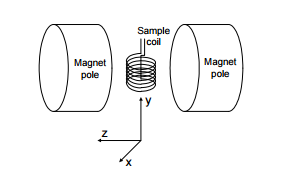
\includegraphics[scale=.4]{Sample_Env.png}
      \caption{The permanent magnetic field is directed along the $+z$ direction while the sample coil (pickup coil) detects magnetization of the sample in along the transverse ($y$) axis. Not shown are the RF coils used to tip the spins from alignment with the permanent field. Figure taken from A Conceptual Tour of NMR Ref. \cite{Concept_Tour}}
      \label{fig:Sample_Env}
\end{figure}
\subsection{T1}
\label{sub:T1_Theory}
When spins flip from $-Z$ to $+Z$ they change energy and must release this energy into the lattice of the material surrounding them, for this reason the time $T_1$ which describes this process is known as the Spin-Lattice Relaxation time. The differential equation describing the $Z$ axis magnetization is:
\begin{equation}
	\frac{dM_z}{dt}=\frac{M_0 - M_Z}{T_1},
\end{equation}
where $M_0$ is the initial magnetization and $T_1$ is the characteristic time we are interested in studying.
Solving for $M_Z(t)$ results in:

\begin{equation}
\label{eq:T1_Fit}
	M_Z(t) = M_0-Ce^{\frac{-t}{T_1}},
\end{equation}
A $\pi$ pulse sets the initial condition as:
\begin{align*}
	M_z(t=0)=-M_0,
\end{align*}
allowing us to solve for $M_Z(t)$:
\begin{equation}
\label{eq:Mz}
	M_Z(t) = M_0(1-2e^{\frac{-t}{T_1}}).
\end{equation}
Unfortunately $M_Z(t)$ is not directly measurable so a $\frac{\pi}{2}$ pulse is applied to the sample a time $\tau$ after the $\pi$ pulse flips the net magnetization along the $Z$ axis into the x-y plane where the spectrometer can detect the magnitude. In this way a measurement of $|M_Z(\tau)|$ is obtained. By varying the delay time $\tau$ data can be collected and fit to Eq. \ref{eq:T1_Fit} in order to determine $T_1$. 

After a $\pi$ pulse we expect $M_Z(t)$ to increase until it reaches its equilibrium value. Thus we expect the range of data for which the measured $|M_Z(t)|$ is decreasing to correspond to $M_Z(t)<0$, and data should be modified for analysis accordingly.

\subsection{T2}
\label{sub:T2_Theory}
The relaxation of spins from the x-y plane to the $Z$ axis is characterized by a time $T_2$ known as the Spin-Spin relaxation time. Unlike $T_1$ processes this does not involve transfer of energy to the surrounding lattice and thus we expect that $T_2<T_1$. The decay of the net magnetization in the x-y plane is known as the Free Induction Decay (FID) and is not solely dependent on $T_2$ processes. Due to field inhomogeneities the spins will precess around the $Z$ axis at different rates ultimately decohering on time scale $T_2$* causing the net x-y magnetization to drop to 0. If $T_2$* is short compared to $T_2$ a measurement of the FID will effectively be a measure of only $T_2$* as the $T_2$ processes will not have had time to become significant.


This issue can be avoided through a two-pulse technique known as spin echo, which forces the precessing spins to recohere allowing measurement of $T_2$. The application of a $\frac{\pi}{2}$ pulse tips the spins into the x-y plane where they begin to precess. Some time $\tau$ later the application of a $\pi$ pulse will reverse the direction of precession of the spins so that at $t=2\tau$ the spins will be coherent resulting in a peak in the signal detected. However this signal will be reduced compared to the amplitude of the FID resulting from the first pulse as spins will have decayed via $T_2$ processes. For an excellent discussion of this see A Conceptual Tour of NMR \cite{Concept_Tour} The difference in amplitude of the first and second FID is the result of spins decaying via $T_2$ processes. By varying $\tau$ and recording the difference in peak amplitudes we can determine $T_2$ based on the following equations.

From Ref. \cite{TeachspinManual} we have that spins tipped into the x-y plane by a $\frac{\pi}{2}$ pulse will decay to the Z axis with the following dependence:
\begin{equation}
M_{x,y}(t)=M_0e^{\frac{-t}{T_2}}
\end{equation}
At $t=0$ we have:
\begin{align}
M_{x,y}(t=0)=M_0
\end{align}
So the difference in the maximum x-y plane magnetization after a time $\tau$ measured as voltage will be:
\begin{equation}
\label{eq:T2_Fit}
\Delta V=M_0(1-e^{\frac{-\tau}{T_2}})
\end{equation}
For an example of $\Delta V$ see Fig. \ref{fig:Typical_T2}

%===============================================================================================
\section{Experimental Procedures}
\begin{figure}[h!]
  \centering
      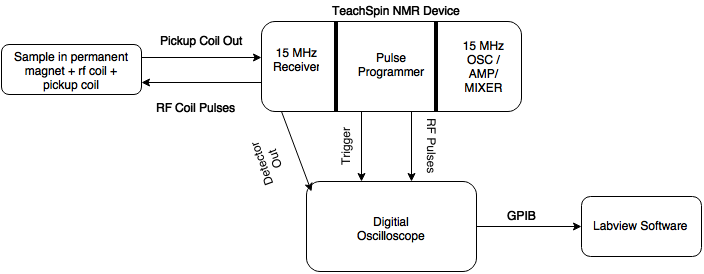
\includegraphics[scale=.4]{NMR_Block_Diagram.png}
      \caption{Block Diagram For the experiment. The TeachSpin device would provide RF pulses to flip the spins and output a clean signal to the oscilloscope from which measurement were made. For a diagram of the sample environment see Figure \ref{fig:Sample_Env}}
      \label{fig:Block_Diagram}
\end{figure}

A TeachSpin Pulsed NMR PS1-D device was used to produce magnetic pulse and amplify the output of the pickup coil. The outputs were monitored with a Tektronix 200 MHz digital storage oscilloscope connected to a computer --via Labview.

Prior to determination of the time constants $T_1$ and $T_2$ the frequency of the rf field was adjusted to the resonant frequency of the system. This was accomplished by minimizing the amplitude of the beat frequency signal of from the rf coil and the excitation applied.

The length of a $\frac{\pi}{2}$ pulse was determined by finding the minimum pulse width that resulted in a maximum of FID amplitude. After this the pulse width of a $\pi$ pulse was determined as the first pulse width value greater than the $\frac{\pi}{2}$ pulse width that caused no signal to be detected by the pickup coil.

\subsection{T1}
Following the theory developed in Section \ref{sub:T1_Theory} a $\pi$ pulse followed by a $\frac{\pi}{2}$ pulse was applied to the sample and the maximum voltage of the resulting peak was recorded along the delay time between peaks. As discussed above data points from the concave up portion of the data curve were taken as the negative values of M$_Z$.

This Voltage was fit to Eq. \ref{eq:T1_Fit} with a least squares method in order to determine $T_1$.
\begin{figure}[h!]
  \centering
      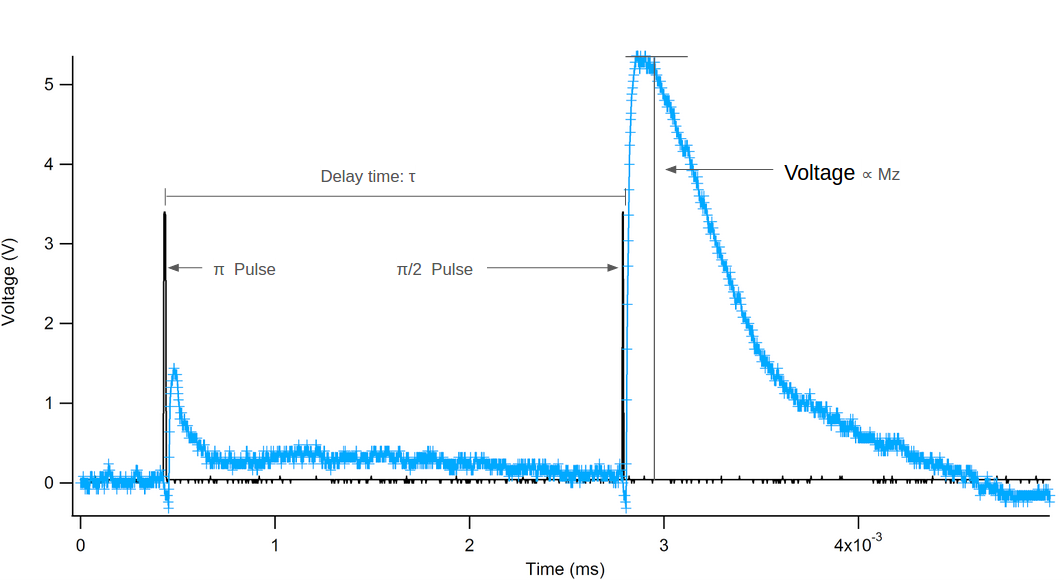
\includegraphics[scale=.3]{Typical_T1_Annotated.png}
      \caption{A typical waveform used to determine $T_1$. The voltage of the peak following the $\pi$ pulse is of interest in order to determine $T_1$. Blue Crosses are spectrometer measurements, solid black line is applied rf pulses.}
      \label{fig:Typical_T1}
\end{figure}
\FloatBarrier
\subsection{T2}
Following the theory developed in Section \ref{sub:T2_Theory} a $\frac{\pi}{2}$ pulse was applied followed by a $\pi$ pulse some time $\tau$ later. $\tau$ was varied and the difference between the two peaks in the resultant waveform was measured as $\Delta V$ and fit to Eq. \ref{eq:T2_Fit}.

\begin{figure}[h!]
  \centering
      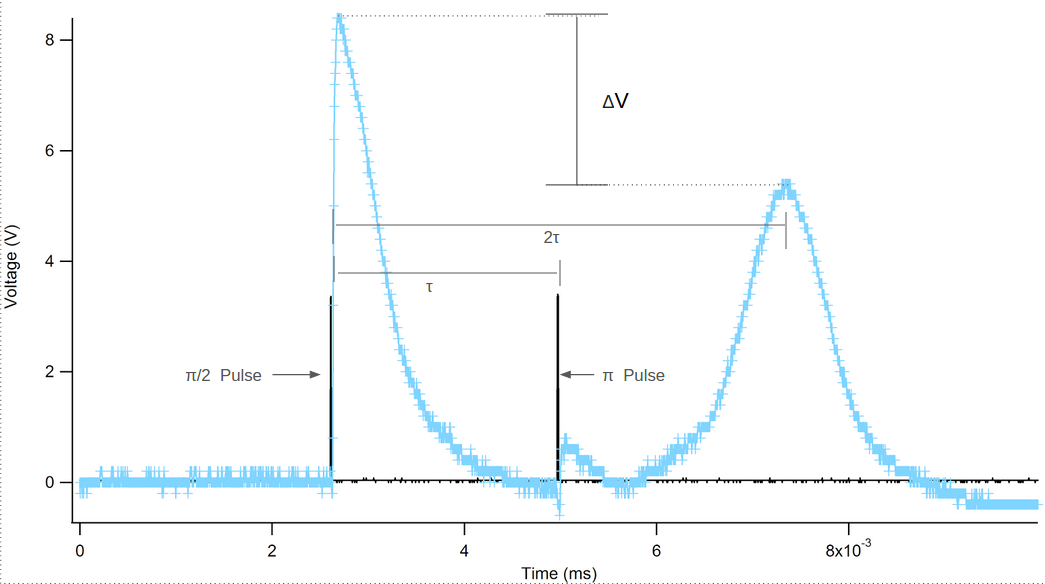
\includegraphics[scale=.3]{Typical_T2_Annotated.png}
      \caption{A typical waveform used to determine $T_2$. The quantity $\Delta V$ is of interest in determining $T_2$. Blue Crosses are spectrometer measurements, solid black line is applied rf pulses.}
      \label{fig:Typical_T2}
\end{figure}
\FloatBarrier

%=================================================================================

\section{Results}
Data was fit to $y_0+Ae^{\frac{-t}{\tau}}$ by a weighted least-squares method. The error in the voltage measurement was determined by $\chi^2$ analysis, as discussed in Sec. \ref{sec:ChiSq}.

\begin{figure}[h!]
  \centering
      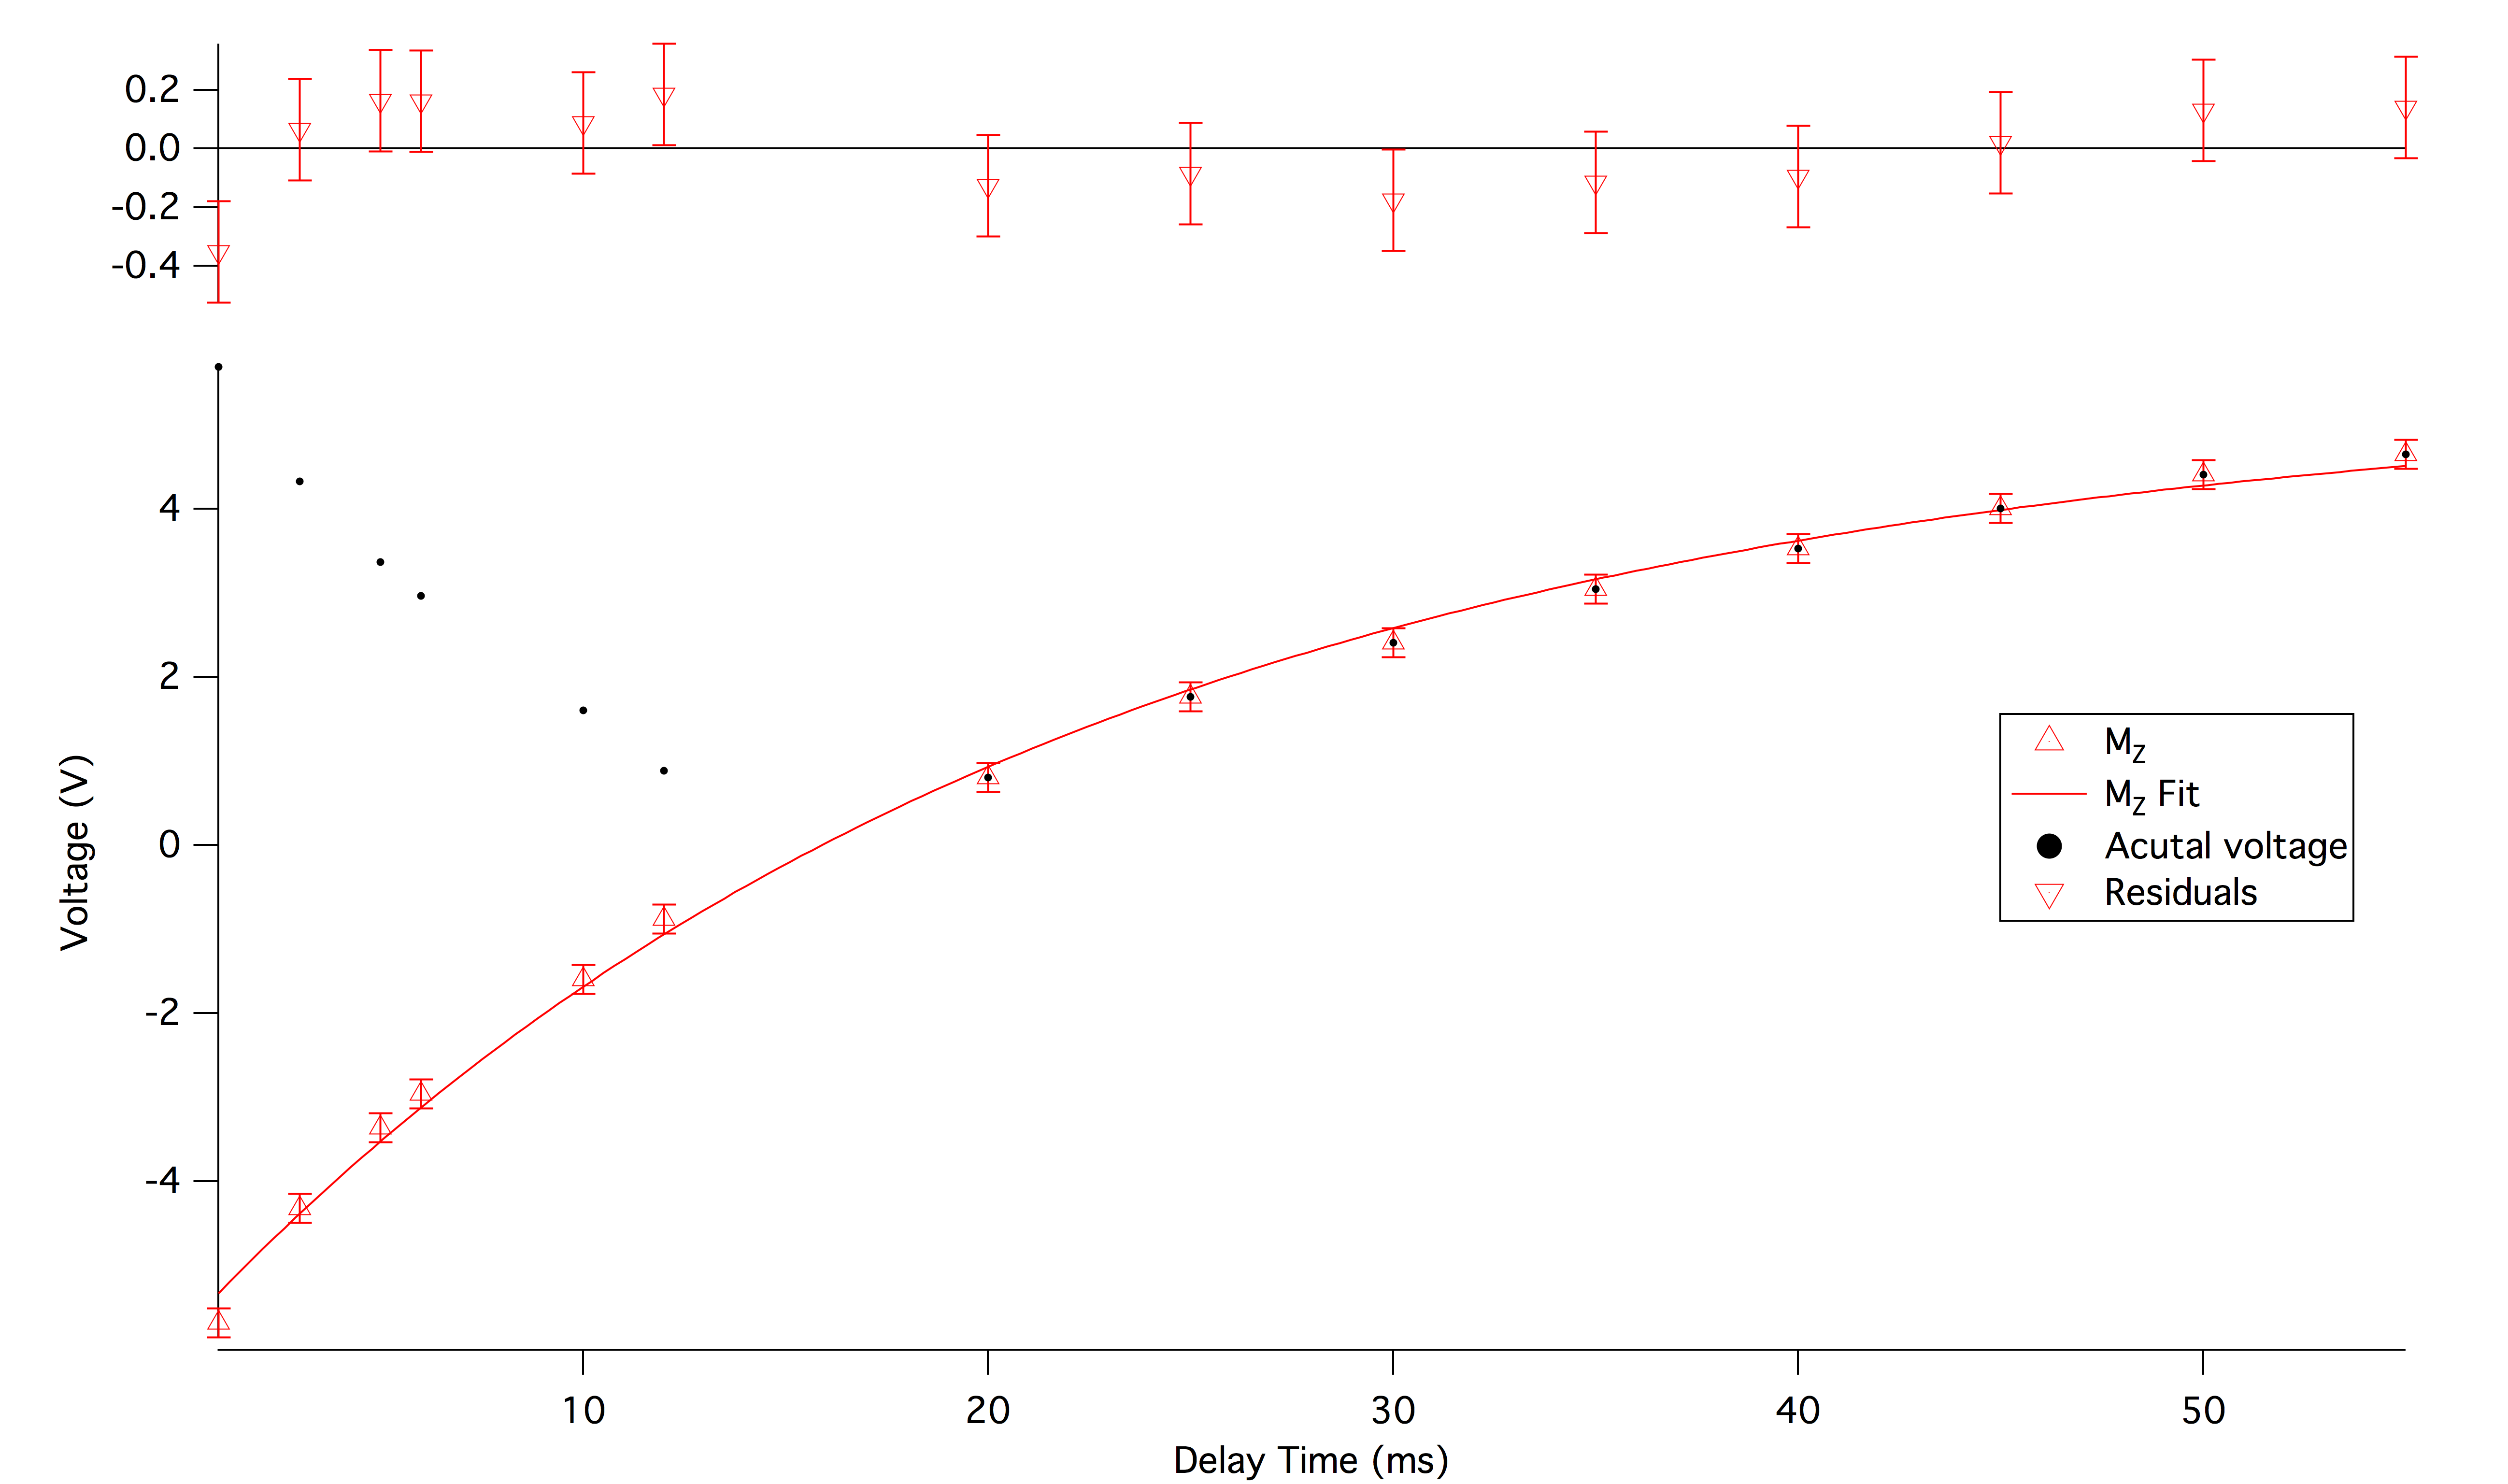
\includegraphics[scale=.3]{T1_Fit_newError.png}
      \caption{{\small Determining $T_1$, note the apparent structure in the residuals, this may indicate a failure of the model to capture multiple $T_1$ times in the sample. Black dots are recorded $\Delta$V, red triangles are the data with decreasing values made negative for reasons described in Section \ref{sub:T1_Theory}}.}
      \label{fig:T1_Fit}
\end{figure}	

\begin{figure}
  \centering
      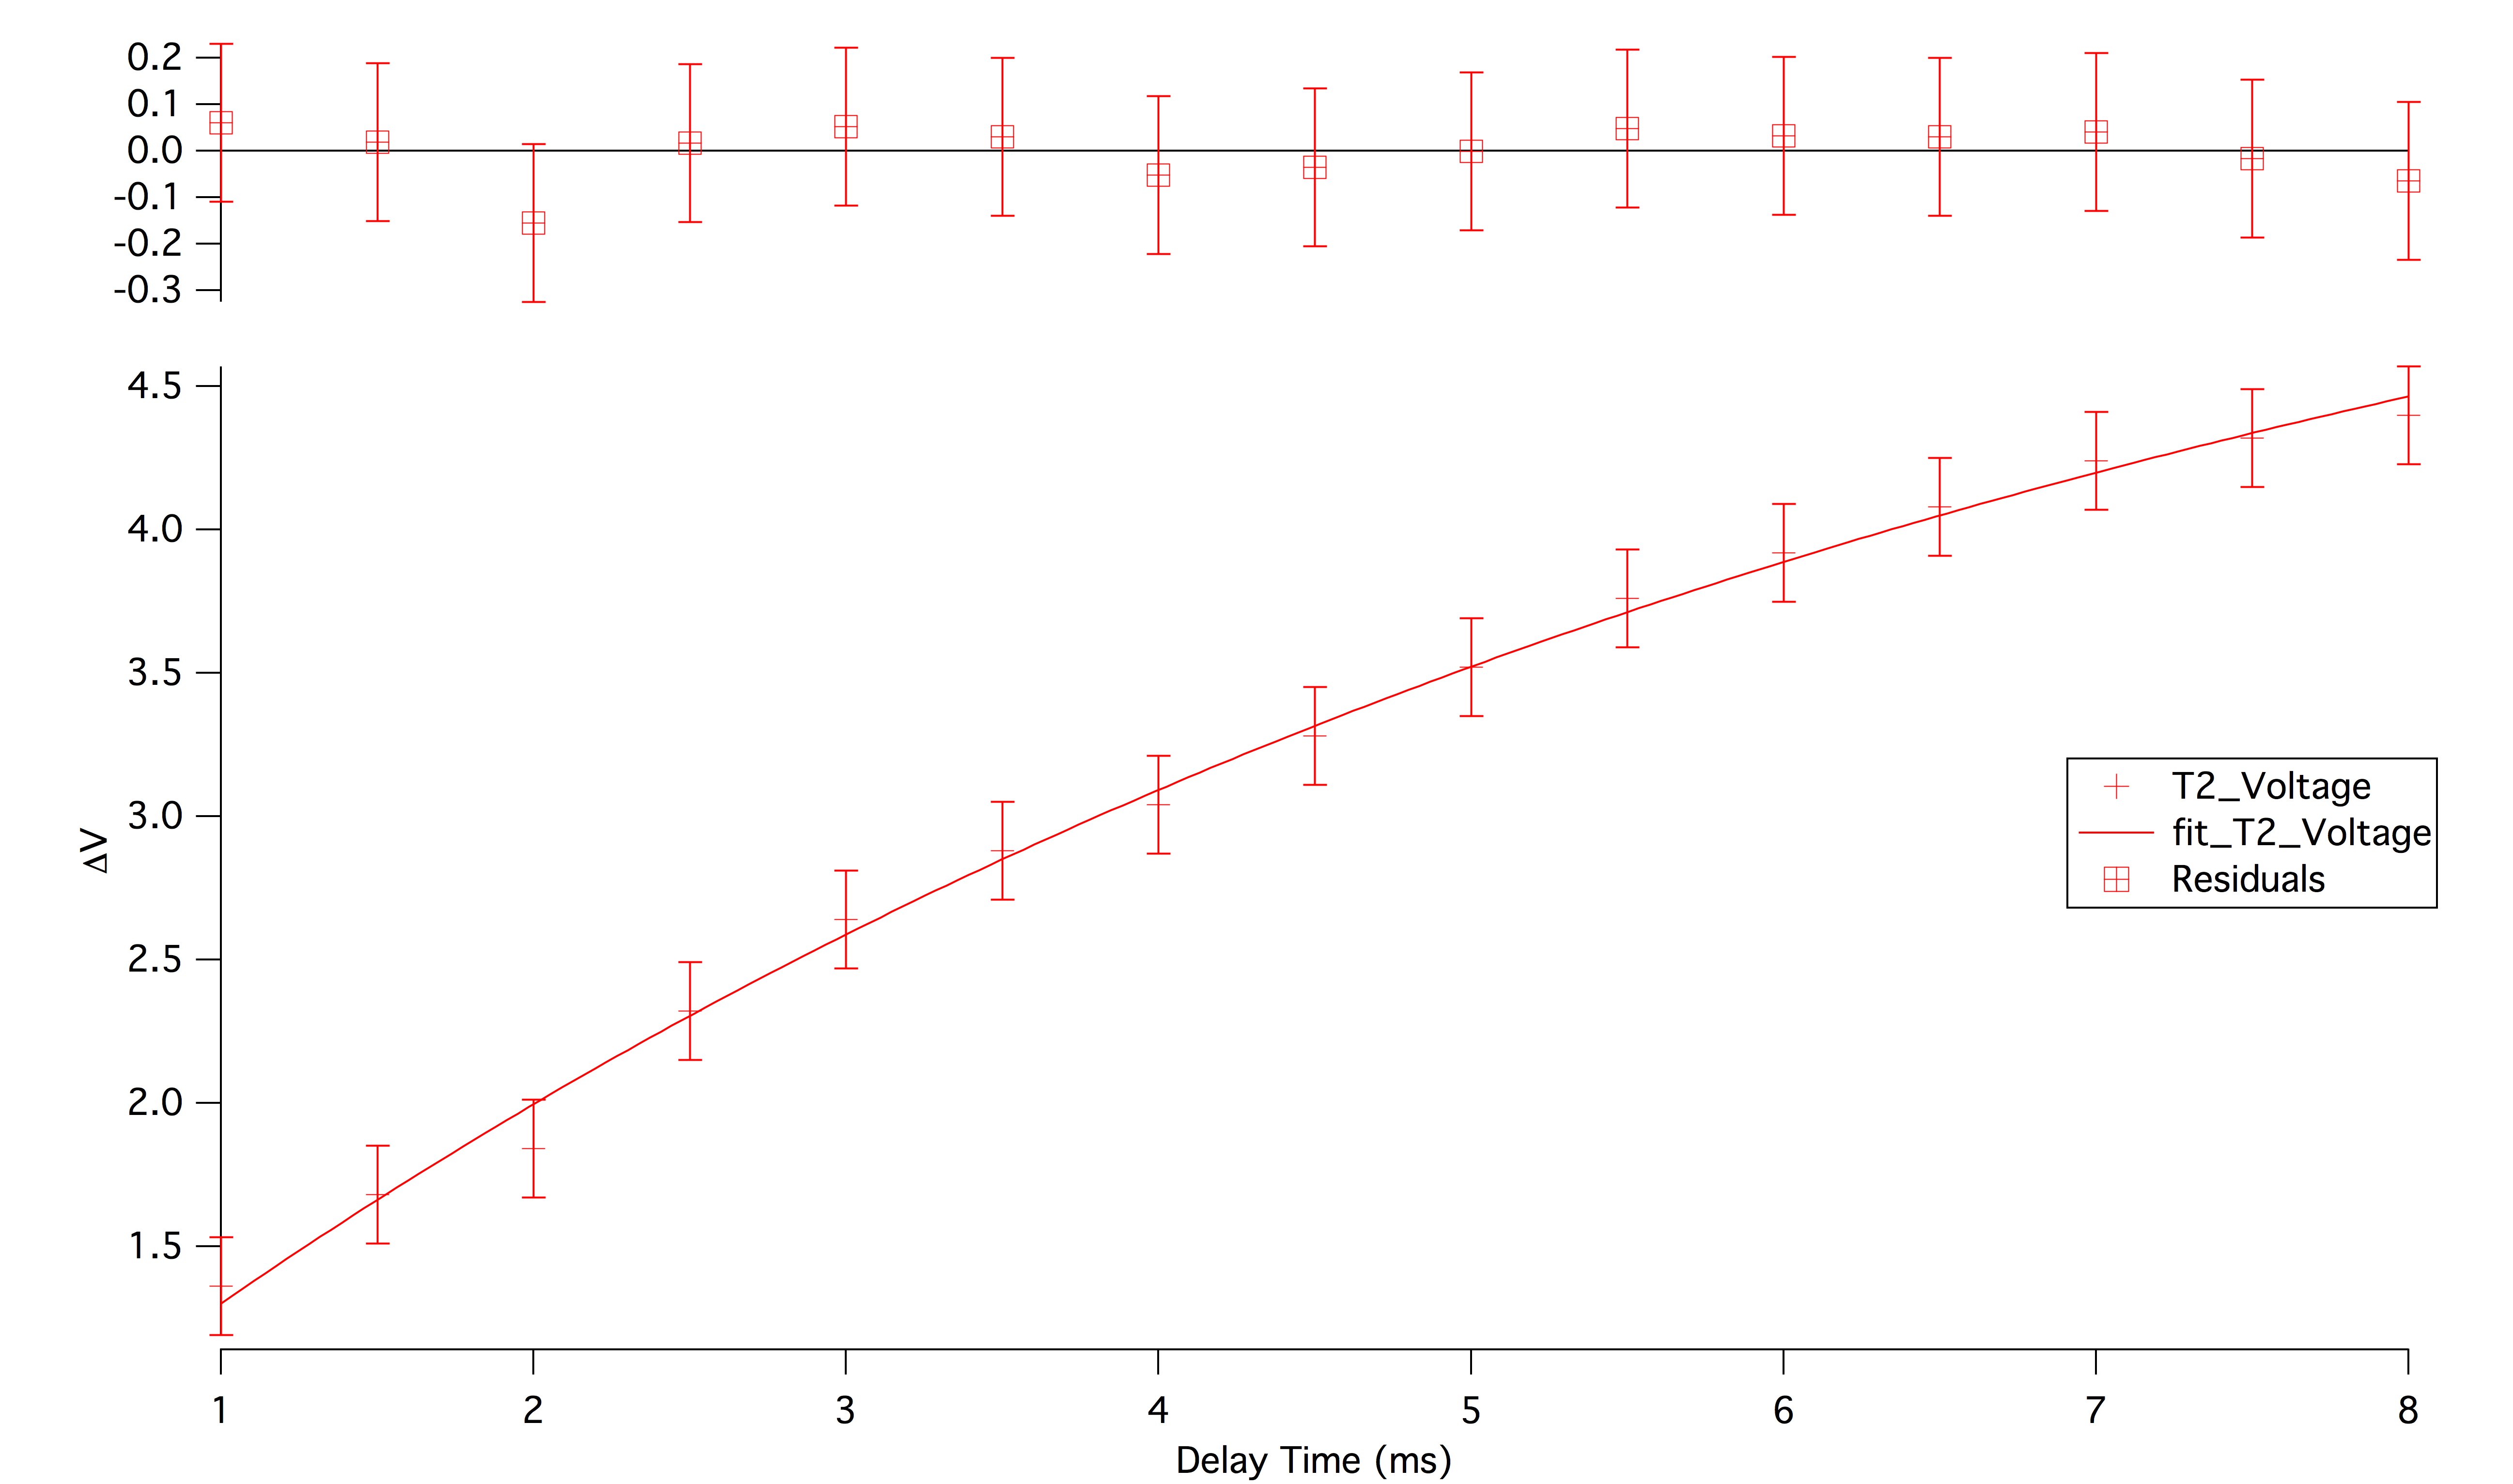
\includegraphics[scale=.3]{T2_Fit_newError.png}
	\caption{Determining $T_2$, note the lack of a trend in the residuals. The error on the data for this plot is same as in Fig. \ref{fig:T1_Fit} however it appears larger due to a reduced y-axis scale. In this data there is no apparent structure to the residuals in contrast to the data for $T_1$}
    \label{fig:T2_Fit}
\end{figure}
\FloatBarrier


\begin{table}[!h]
\label{Result_Table}
\begin{center}
	\begin{tabular}{|c|c||c|}\hline
		Quantity & This Work & Bianchini and Coffey \\ \hline\hline
		$T_2^*$ & .47 ms &  N/A \\ \hline
		$T_2$ & 6.23 $\pm$ .55 ms &  15.7 $\pm$ .01 ms \\ \hline
		$T_1$ & 21.68 $\pm$ 1.2 ms &  25.4 $\pm$ .07 ms\\ \hline
	\end{tabular}
		\caption{Values from this work and from Ref. \cite{Bianchini}. The results from this work and that of Bianchini and Coffey are in the same order of magnitude, as good agreement as could be expected for mineral oil, a non-standardized substance.}
		\end{center}
	\end{table}
Values the time constants were determined from these fits and are presented in Table \ref{Result_Table}. As expected $T_2^*$ is significantly smaller than $T_2$. Also note that $T_1$ is $\sim$3x more than $T_2$. This is sensible as $T_1$ involves a transfer of energy to the lattice while $T_2$ does not involve a transfer of energy.
Our values $T_1$ and $T_2$ are on the same order of magnitude as as those found by Bianchini and Coffey, that they are several standard deviations apart is not significant as Mineral Oil is not a standardized substance.

\subsection{Uncertainty Budget}
\begin{table}[!h]
	\begin{center} 
		\begin{tabular}{|c|c|c|c|} \hline 
			Source & Quantity&  Error in Quantity  & Propagated Error  \\ \hline \hline
			Model Error/Fitting Error& $T_1$ &  & 1.2 (ms)\\ \hline
			Model Error/Fitting Error& $T_2$ & & .55 (ms)\\ \hline
			Pulse Width&  & 5\% & .05 \%\\
			\hline
		\end{tabular}
        \caption{Uncertainty Budget for this work. The model for $T_1$ in particular may not be capable of fully describing the system. For more information see \ref{sec:ChiSq}.}
	\end{center}
\end{table}
Due to the use of oscilloscope cursors to determine the voltages for determining $T_1$ and $T_2$ the original error values were estimated as $\pm .05$ V. This error was later increased to $\pm .17$ V as a consequence of $\chi^2$ analysis.

 The inability to determine the exact length of a $\frac{\pi}{2}$ and $\pi$ pulses was also a source of error. However this effect was minimal compared to other factors as investigation found that a $10\%$ deviation from the best guess for a $\frac{\pi}{2}$ pulse only resulted in a $1\%$ difference in the FID magnitude.
\subsection{$\chi^2$ analysis}
\label{sec:ChiSq}
The data was first fit with errors in the data of $\pm .05$V however this produced high $\tilde{\chi}^2$ indicating a lower than necessary estimate of errors. As the $\tilde{\chi}^2$ for $T_1$ was originally 12.17 the error for that was re-estimated as $\sigma=.05*\sqrt{12}$. This produced the $\chi^2$ analysis in Table \ref{table:ChiSq}.

\begin{table}[!h]

	\begin{center}
		\begin{tabular}{|c|c|c|c|c|} \hline
			Quantity & $\chi^2$&Deg Freedom&$\tilde{\chi}^2$  &  Probability \\ \hline \hline
			$T_1$ & 11.16 & 14 & .797 &  67 \%   \\ \hline
			$T_2$ & 18.55 & 15 & 1.23 & 14 \%   \\ \hline
		\end{tabular} \\
		\caption{Probabilities were determined from Ref. \cite{TaylorError}}
        \label{table:ChiSq}
	\end{center}
\end{table}


Even with re-estimated error the $\chi^2$ analysis indicates that our models are not fully capturing the system. The most likely reason for this is that the sample is best described by multiple $T_1$ and $T_2$ values. This would occur if local field inhomogeneities caused nuclei in the sample to have different field environments resulting in their having a different characteristic time scale for relaxation than the rest of the sample. One piece of evidence for this theory that there are multiple times is the structure in the residuals of $T_1$, Fig. \ref{fig:T1_Fit}. With the residuals $>0$ for data points with $V<0$ and $>0$ for $V>0$ we might conclude that the calculate $T_1$ time is actually a convolution of two times, one shorter and once longer than the calculated value. 

It is interesting to note that there is no equivalent structure in the residuals of $T_2$ despite a similar number of data points being used. This may indicate that there is only one $T_2$ for the sample however more investigation is necessary.
\section{Conclusions}
A model was developed that predicted an exponential decay type return towards equilibrium magnetization when spins had their direction changed by an oscillating rf field. This model predicted that the system would have two characteristic times $T_1$ and $T_2$ corresponding to spins relaxing from the $-Z$ direction and x-y plane to the $+Z$ direction. Data was fitted to these models in order to determine values of $T_1=21.68\pm 1.2$ ms and $T_2=6.25\pm .55$ ms. As predicted we found $T_2<T_1$ however, $\chi^2$ analysis and the residuals from the fits indicate that this may not be a full description of the system. In particular we speculate that there are multiple values for $T_1$ and $T_2$ perhaps due to field inhomogeneities due to the strength of the permanent magnet used. Further work might include developing a model that incorporates multiple $T_1$ and $T_2$ times and fitting the data to this model.
\section{Acknowledgements}
Pete Sinn was invaluable as a Lab Partner when performing this experiment.

\begin{thebibliography}{99}
\bibitem{NMR_Uses} NMR Applications, Michigan State University 900 MHz NMR Facility, https://www2.chemistry.msu.edu/facilities/nmr/900MHz/MCSB\_NMR\_applications.html
\bibitem{Pake} George E. Pake, "Nuclear Magnetic Resonance in Bulk Matter," Physics Today Oct. 1993, page 46.  
\bibitem{Concept_Tour} Barbara Wolff-Reichert, Conceptual Tour of PNMR, 2008 
\bibitem{TeachspinManual} Teachspin Instructional Pulsed NMR Apparatus Manual, Department of Physics and Astronomy, Knoxville, TN
\bibitem{TaylorError} J.R. Taylor, {\it Introduction to Error Analysis}, (University Science Books, Sausalito, 1997)
\bibitem{Bianchini} L. Bianchini, L. Coffey, Physics Department, Brandeis University, NMR Techniques Applied to Mineral Oil, Water, and Ethanol (2010)


\end{thebibliography}
\end{document}